\chapter{Supervised Machine Learning}
A machine is said to learn if, when tackling a task, it is able to improve its own
performance through experience.
\begin{itemize}
	\item Task $T$: the problem we are trying to solve, e.g., predict the cancer risk of a patient
	\item Experience $E$: the experience on the task provided to the model, e.g., some dataset
	\item Performance $P$: a measure of success, e.g., the success rate in predicting cancer
	\item Model $F$: a function $f$ solving the task with a learning algorithm $A$
\end{itemize}

\begin{table}[h]
\centering
\begin{tabular}{|p{4cm}|p{4cm}|p{7cm}|}
\hline
\textbf{Task} & \textbf{Predict} & \textbf{Example} \\ \hline
Binary classification & one of two discrete labels & Is the patient at high risk of developing cancer, or not? \\ \hline
Multilabel classification & any of several discrete labels & Of all the possible syndromes, which is the patient going to develop? \\ \hline
Multiclass classification & one of several discrete labels & The student is going to major in...? \\ \hline
Regression & a continuous label & The student's grade is going to be...? \\ \hline
\end{tabular}
\caption{Types of supervised learning tasks}
\label{tab:supervised-tasks}
\end{table}

\section{Experience or not}
Models are not developed to aid on known experiences, rather on \textbf{unknown} ones.
The performance of a model can't be uniquely measured on its performance on the given experience, but rather on novel experiences which the model was not preview to. We want to achieve a low generalization error.

\begin{itemize}
   \item \textbf{Optimization}\\
   Maximizes performance on the
   given experience $E$: optimization
   performance
   \item \textbf{Machine Learning}\\
   Maximizes performance on the
   given, and expected non-given,
   experience $E$ and $\bar{E}$: generalization performance
\end{itemize}

If we do not know the non-given experience $\bar{E}$ how can we ever expect to be effective on it?\\
\textbf{Equal distribution assumption}. It is assumed that the given experience $E$, and the non-
given experience $\bar{E}$ are sampled from the same distribution $Pr^E$.\\
Given a learning algorithm $A$, can I always expect the performance to transfer?\\
\textbf{No.}

Sampling from the data distribution is a random process, and the resulting
models learned end up erring in terms of:
\begin{itemize}
	\item Bias: the expected performance decrease w.r.t. the best model
	\item Variance: the variance with respect to different samples
\end{itemize}
Ideally, we want to have learning algorithms with low enough bias and variance.

\newpage
\section{Improper models}
\begin{paracol}{2}
   
   There are two categories of improper models:
   \begin{itemize}
      \item Underfit. High bias, high variance.
      Models which have poor
      performance, regardless of samples.
      They have not learnt enough!

      High variance, low bias. Models which ought to improve their performance on the given experience $E$
      \item Overfit. Low bias, high variance.
      Models which have overfit on the
      given experience, and ought to
      improve their generalization
      performance. They have learnt too
      much!

      Low variance, high bias. Models which ought to improve their generalization performance on the unknown experience $\bar{E}$
   \end{itemize}

   \switchcolumn

   \begin{figure}[htbp]
      \centering
      \includegraphics{images/10/biasvariance.png}
      \caption{Bias (red) and variance (blue) as a decomposition of model performance}
      \label{fig:10/biasvariance}
   \end{figure}

\end{paracol}

\begin{figure}[htbp]
   \centering
   \includegraphics[width=0.35\columnwidth]{images/10/fitting.png}
   \includegraphics[width=0.45\columnwidth]{images/10/fitted.png}
   \caption{Two models approximating a dataset: one model has too
low a capacity and underfits the data (in red), while another
has too high a capacity and overfits the data (in blue).
These are opposed to a well-fitted model (in green) which
generalizes well, without being too strict and leaving some space for variance in data.}
   \label{fig:10/fitting}
\end{figure}


\section{Searching for models}
\begin{itemize}
	\item \textit{Tackling the generalization gap.} Data-based strategies to maximize generalization performance
	\item \textit{Performance evaluation.} How to measure model performance/error
	\item \textit{Parameterization.} Exploring the space of models
\end{itemize}


We design two phases in the model search:
\begin{itemize}
   \item \textbf{Model selection}\\
   A learning phase wherein, among all possible models in a model
space $\mathcal{F}$, we select a model $f$
   \item \textbf{Model Validation}\\
   A learning phase wherein we estimate the generalization performance (error) of the selected model $f$
\end{itemize}
Model validation cannot affect model selection: it only goes one way, from selection to
validation. Thus, we need to incorporate in model selection some strategy to avoid
under/overfitting

\newpage
\subsection{Data Partitioning}

The standard approach is model agnostic: we can apply this to any learning algorithm or family of models we want. We operate a tripartite partitioning of $(X, Y)$:

\begin{paracol}{2}

\begin{itemize}
    \item \textbf{Training dataset} $(X^{tr}, Y^{tr})$: search through the models' space $\mathcal{F}$
    
    \item \textbf{Validation dataset} $(X^{vl}, Y^{vl})$: guesstimate the generalization performance of candidate models $f_1, \dots, f_k$
    
    \item \textbf{Test dataset} $(X^{ts}, Y^{ts})$: estimate the generalization performance of the selected model $f_i$
\end{itemize}

\switchcolumn

\begin{figure}[htbp]
\centering
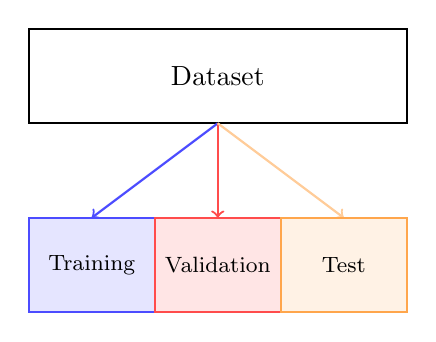
\begin{tikzpicture}[scale=0.8]
    % Main dataset
    \draw[thick] (0,2) rectangle (6,3.5);
    \node at (3,2.75) {Dataset};
    
    % Arrows
    \draw[->, thick, blue!70] (3,2) -- (1,0.5);
    \draw[->, thick, red!70] (3,2) -- (3,0.5);
    \draw[->, thick, orange!40] (3,2) -- (5,0.5);
    
    % Training set
    \draw[thick, blue!70, fill=blue!10] (0,0.5) rectangle (2,-1);
    \node at (1,-0.25) {\footnotesize Training};
    
    % Validation set
    \draw[thick, red!70, fill=red!10] (2,0.5) rectangle (4,-1);
    \node at (3,-0.25) {\footnotesize Validation};
    
    % Test set
    \draw[thick, orange!70, fill=orange!10] (4,0.5) rectangle (6,-1);
    \node at (5,-0.25) {\footnotesize Test};
    
\end{tikzpicture}
\caption{A partition of the dataset (in black) in training (blue), validation (red), and test (beige).}
\label{fig:data-partition}
\end{figure}

\end{paracol}

\begin{table}[h]
\centering
\begin{tabular}{|l|l|l|l|}
\hline
\textbf{Task} & \textbf{Training} & \textbf{Validation} & \textbf{Test} \\ \hline
Disease diagnosis & Biology lectures & Homework & Exam \\ \hline
Learning a language & Duolingo & Exchange student & Living abroad \\ \hline
Pandemic diffusion & Black plague & Ebola & Covid \\ \hline
\end{tabular}
\caption{Analogy between data partitioning and real-world learning}
\label{tab:data-partition-analogy}
\end{table}

\subsubsection{Partitioning the dataset}

How to partition the dataset properly?
\begin{itemize}
	\item \textbf{Size} - Test and validation set of
similar size, training set of much
larger size, e.g., a ratio of 4:1. Some
learning algorithms are more data-
hungry, so this is a starting baseline.
	\item \textbf{Distribution} - Ideally, same
distribution for all three datasets.
Random stratified sampling is used
\end{itemize}

\begin{figure}[htbp]
   \centering
   \includegraphics{images/10/partition.png}
   \caption{Partitioned data}
   \label{fig:10/partition}
\end{figure}

\subsection{Model selection}

There are two key model selection strategies: \textbf{hold-out} and \textbf{cross-validation}.

{\textbf{Hold-out} leverages the three-blocks partition train-validation test.\ns
\begin{itemize}
	\item Learn candidate models $f_1,\dots f_k$ on the training set
	\item Evaluate them on the validation set
	\item Estimate the generalization error on the test set
\end{itemize}}

\newpage
\textbf{K-fold Cross-validation} aims at run multiple times the hold-out strategy, to increase the size of the validation set. We partition a given set of data, e.g., the training dataset, in $k$ blocks (folds). In each fold, one block acts as validation set, while the other $k-1$ blocks act as training set. We repeat this $k$ times, each time changing the validation block.

\begin{paracol}{2}
   
   \colfill
   Stretching hold-out, we aim to further increase the size of the validation set.
   We partition a given set of data, e.g., the training dataset, in two folds:
   \begin{itemize}
      \item in set 1, block 1 is a training dataset, block 2 is the validation dataset
      \item in set 2, block 1 is a training dataset, block 2 is the validation dataset
   \end{itemize}
   Now I can learn and guesstimate a model
   $f_i$ on both folds!

   This is called \textbf{2-fold cross-validation}, but we can generalize it to $k$ folds.
   \colfill
   
   \switchcolumn

   \begin{figure}[htbp]
      \centering
      \includegraphics{images/10/2fold.png}
      \caption{A set partitioned in two blocks, and the resulting folds. In each fold, a block acts as validation set (in red), and the other as training set (in blue).}
      \label{fig:10/2fold}
   \end{figure}

\end{paracol}

\begin{figure}[htbp]
   \centering
   \includegraphics{images/10/kfold.png}
   \caption{A set partitioned in $k$ blocks, and the resulting folds. In each fold, a block acts as validation set (in red), and the other as training set (in blue).}
   \label{fig:10/kfold}
\end{figure}

\section{Performance evaluation}

With proper partitioning, we are now able to feed experiences (data) to the candidate
models $f_1, \dots, f_k$ we wish to select. How do we evaluate them?

\textbf{Classification} - Classification tasks generally aim to measure a Hamming distance ($\ominus$)
between the gold labels, and the labels given by the model. \ul{Either measured as error or performance.}

Reminder: we indicate the vector of n gold labels with $Y \in y$, the model of interest $f$ with $f$, its prediction on an instance $x^i$ with $f(x^i)$, and the indicator function with $\mathbb{1}$.

\begin{table}[h]
\centering
\begin{tabular}{|l|l|p{8cm}|}
\hline
\textbf{Task} & \textbf{Measure} & \textbf{Formulation} \\ \hline
Binary, Multiclass & Accuracy & $\displaystyle\frac{1}{n}\sum_{i=1}^{n} \mathbb{1}(Y_i = f(x^i))$ or $1 - \textit{Error rate}$ \\ \hline
Binary, Multiclass & Error rate & $\displaystyle\frac{1}{n}\sum_{i=1}^{n} \mathbb{1}(Y_i \neq f(x^i))$ or $1 - \textit{Accuracy}$ \\ \hline
Multilabel & Jaccard similarity & $\displaystyle\frac{1}{n}\sum_{i=1}^{n} \frac{Y_i \cap f(x^i)}{Y_i \cup f(x^i)}$ \\ \hline
Multilabel & Hamming error & $\displaystyle\frac{1}{n}\sum_{i=1}^{n} 1 - (Y_i \ominus f(x^i))$ \\ \hline
\end{tabular}
\caption{Performance measures for classification tasks}
\label{tab:classification-measures}
\end{table}



\newpage
\subsection{Confusion Matrix}

\begin{paracol}{2}
   
   \colfill
   In some binary cases, one label $y$ is for us of interest (positive label), e.g., patients we predict will have cancer, while the other is not (negative label). We can construct a \textit{confusion matrix} out of the predictions $f(x^i)$ of the model, that we can then leverage to define more performance measures.
   \colfill
   
   \switchcolumn

   \begin{figure}[htbp]
      \centering
      \includegraphics{images/10/confusion1.png}
      \caption{A confusion matrix: columns defined by the gold labels $Y$, and rows defined by the predicted labels $f(X)$.}
      \label{fig:confusion-matrix}
   \end{figure}
   
\end{paracol}

\begin{table}[h]
\centering
\begin{tabular}{|l|l|p{5cm}|p{7cm}|}
\hline
\textbf{Task} & \textbf{Measure} & \textbf{Formulation} & \textbf{Description} \\ \hline
Binary & Precision & $\displaystyle\frac{tp}{tp + fp}$ & Of all the positive predictions, how many, in proportion, are correct? \\ \hline
Binary & Recall & $\displaystyle\frac{tp}{tp + fn}$ & Of all the positive instances, how many, in proportion, have been correctly predicted? \\ \hline
Binary & $f1$-score & $h(\text{precision}, \text{recall})$ & Harmonic mean of precision and recall \\ \hline
Binary & Accuracy & $\displaystyle\frac{tp + tn}{tp + tn + fp + fn}$ & Accuracy \\ \hline
\end{tabular}
\caption{Binary classification performance measures from confusion matrix}
\label{tab:binary-measures}
\end{table}

\begin{paracol}{2}
   
   \colfill
   Confusion matrices are limited in their weighting, as any entry, e.g., true positives ($tp$), has a unitary weight in all performance measures. Yet, in some cases, some false weigh heavier than others, e.g., diagnosing a false positive cancer is far worse than diagnosing a false negative. Thus, we introduce the cost matrix, holding one weight per each entry in the confusion matrix, weighing it in performance measures.
   \colfill

   \switchcolumn

   \begin{figure}[htbp]
      \centering
      \includegraphics{images/10/confusion2.png}
      \caption{Confusion Matrix having weights for each entry, forming a cost matrix.}
      \label{fig:10/confusion2}
   \end{figure}
\end{paracol}

For non-binary classification tasks, we can set one label as positive, and all others as negative, and build multiple confusion matrices, one per label, and then aggregate the results.

\subsection{ROC Curve}

\begin{paracol}{2}
   
   Among all possible model solving binary
   classification tasks, some do not compute
   a binary label per se, rather a score or
   probability $\alpha$ of a label.
   We need to to try multiple thresholds $\tau$, each yielding different labellings.
   We may plot these results in a \textbf{ROC curve}.

   \switchcolumn

   \begin{figure}[htbp]
      \centering
      \includegraphics{images/10/roc.png}
      \caption{Points are just threshold IDs}
      \label{fig:10/roc}
   \end{figure}
\end{paracol}

There are some points of interest in the ROC curve:
\begin{itemize}
   \item $(0,1)$ - \textbf{Perfect classifier} - no false positives, all true positives
   \item $(1,0)$ - \textbf{Worst classifier} - all false instances are classified as positive, none of the positive instances is classified as positive
   \item $(1,1)$ - \textbf{All positive classifier} - classifies all instances as positive, yielding all true positives, but also all false positives
   \item $(x,x)$ - \textbf{Random classifier} - the diagonal line from $(0,0)$ to $(1,1)$
   \item $(x,x-\sigma)$ - \textbf{Worse than random classifier} - any point below the random classifier, this yields more errors than correct predictions
   \item \textbf{Area under the curve (AUC)} - the area under the ROC curve, a measure of performance. $0.5$ is random, $1$ is perfect.
\end{itemize}

\framedt{Multiple Labels}{
   What happens in case of multiple labels? We can build one ROC curve per label, setting it as positive, and all others as negative. Then, we can average the AUCs of each label to get a final performance measure.
}

\section{Regression}

Unlike classification tasks, regression tasks aim to predict continuous labels. Thus, we need different performance measures, we cannot count ``positive'' vs ``negative'' predictions.

Typical regression performance measures are:
\begin{itemize}
   \item Mean Squared Error (MSE) - Mean error per instance, squared
   \item Max Squared Error (MaxSE) - Maximum error among all instances, squared
   \item R Squared ($R^2$) - Error over default model, where for default model we mean the average of all labels, so the error is the variance of the labels
   // TODO add formula
   % Proportion of variance explained by the model
\end{itemize}